\documentclass[10pt]{beamer}

\usepackage{amsfonts}
\usepackage{subfiles}
\usepackage[T2A]{fontenc}
\usepackage[utf8]{inputenc}
\usepackage[russian]{babel}

\usepackage{amsmath, amsfonts, amssymb, amsthm, mathtools, mathrsfs}
\usepackage{wasysym, dsfont}
\usepackage{graphicx}
\usepackage{float}
\usepackage{wrapfig}
\usepackage{subcaption}
\usepackage{multirow}
\usepackage{caption}
\usepackage{subcaption}
\usepackage{longtable}
% \usepackage{subfigure}

\usepackage{multicol}
\DeclareMathOperator*{\argmax}{\arg\!\max}
\DeclareMathOperator*{\argmin}{\arg\!\min}

\mode<presentation>
{
	\usetheme{boxes}
	\beamertemplatenavigationsymbolsempty
	
	\setbeamertemplate{footline}[page number]
	\setbeamersize{text margin left=1.5em, text margin right=2.0em}
}
\newcommand\blfootnote[1]{%
	\begingroup
	\renewcommand\thefootnote{}\footnote{#1}%
	\addtocounter{footnote}{-1}%
	\endgroup
}
\newcommand\FontUP{\fontsize{12}{12}\selectfont}


\title[]{Обучение взаимосвязанных информативных представлений в задаче генерации образов}
\author{Охотников Никита Владимирович\\ Научный руководитель: к.ф.-м.н. Исаченко Р.В.}

\institute{Кафедра интеллектуальных систем ФПМИ МФТИ\\
				Специализация Интеллектуальный анализ данных\\
				Направление: 03.03.01 Прикладные математика и физика}
\date{2024}


\begin{document}

\begin{frame}
  \titlepage
\end{frame}


\begin{frame}
	\frametitle{Введение}
	Исследуется задача поиска наилучшего дополнения образа --- множества взаимосвязанных элементов --- элементами конечной коллекции.
	\begin{block}{Проблемы}
		\begin{itemize}
			\item Взаимосвязь элементов в образе имеет неизвестную структуру.
			\item Точное решение задачи дополнения требует полного перебора.
		\end{itemize}
	\end{block}
	\vfill
	\begin{block}{Задача}
			Предложить эффективный приближенный алгоритм дополнения образа несколькими элементами.
	\end{block}	

	\vfill
	\begin{block}{Предлагается}
		На основе известной функции оценки образа построить функцию для генерации зависимых скрытых представлений элементов, использующихся далее для выбора элементов дополнения
	\end{block}	
\end{frame}


\begin{frame}
	\frametitle{Постановка задачи дополнения образа}
%		\begin{block}{Основные понятия и обозначения}
			\begin{itemize}
				\item Основная единица данных -- \textit{объект} или \textit{элемент}, множество векторных представлений всех объектов -- $\mathcal{X}\subset \mathbb{R}^d$.
%				\item Далее под объектом $X\in \mathcal{X}$ будем понимать его векторное представление $X\in\mathbb{R}^d$.
%				
%				\item Каждый объект $X\in\mathcal{X}$ есть пара $X = (I, T)$ из соответственно изображения и текстового описания.  
				\item Непустые подмножества множества элементов $O = \{X_i\}_{i=1}^k\subset \mathcal{X}, O\neq\{\O\}$ будем называть \textit{образами}. Множество образов обозначим $\mathcal{O}$.
				\item Для образов введем функцию \textit{оценки} или \textit{совместимости} элементов: 
				$$\mathcal{S}:~2^\mathcal{X}\longrightarrow [0,1], ~~~\forall O \in \mathcal{O}:~\mathcal{S}(O) > 0.$$
%			\end{itemize}
%		\end{block}					
%\end{frame}


%\begin{frame}
%	\frametitle{Постановка задачи}
%	\begin{block}{Задача дополнения образа}
%		\begin{itemize}
			\textbf{Дано:}\\
			$O_n\in\mathcal{O}, ~|O| = n$ --- исходный образ \\
			$k \in \mathbb{N}, ~k$ --- количество элементов дополнения \\	
			
			\textbf{Требуется:}\\
			Найти наилучшее в смысле максимизации функции оценки $\mathcal{S}$ дополнение образа $O_n$  $k$ элементами $\{\hat{X_i}\}_{i=1}^k\subset \mathcal{X}$ т.е. решить следующую оптимизационную задачу
			$$\{\hat{X_i}\}_{i=1}^k= \argmax_{\{X_i\}_{i=1}^k\subset\mathcal{X}} \mathcal{S}\left(O_n\cup\{X_i\}_{i=1}^k\right)$$
%			
%			Точное решение для известной $\mathcal{S}$: полный перебор всех подмножеств $\mathcal{X}$ размера $k$.\\
%			Асимптотика: $|\mathcal{X}|^k$ вызовов функции $\mathcal{S}$
		\end{itemize}
%	\end{block}					
\end{frame}


\begin{frame}
	\frametitle{Теоретическая часть}
	\begin{itemize}	
	 	\item Примем функцию оценки $\mathcal{S}$ известной. (В эксперименте будем рассматривать предобученную модель OutfitTransformer\footnote{\url{https://doi.org/10.48550/arXiv.2204.04812}}).
	    \item Для задачи дополнения 
	    $$\{\hat{X_i}\}_{i=1}^k= \argmax_{\{X_i\}_{i=1}^k\subset\mathcal{X}} \mathcal{S}\left(O_n\cup\{X_i\}_{i=1}^k\right)$$
	    существует 2 глобальных подхода 
	    \begin{enumerate}	
	    	\item Дискретный -- оптимизация полного перебора
	    	\item Непрерывный -- решение некоторой связанной задачи в непрерывном множестве и выбор ближайших к решению элементов $\mathcal{X}$
	    \end{enumerate}
	   \end{itemize}
\end{frame}


\begin{frame}
%	\frametitle{Дополнение образа}
	\frametitle{Дискретный подход}
%	\begin{block}{Дискретный подход}
		\begin{itemize}
			\item Решение задачи приближенным перебором
			\item Бейзлайн: жадные алгоритмы
			\begin{itemize}
				\item[<<1-step>>] $X_1 = \argmax\limits_{X\in\mathcal{X}}{\mathcal{S}(O_n\cup X)},~\dots , X_k = \argmax\limits_{X\in\mathcal{X}\setminus \bigcup\limits_{i=1}^{k-1} X_i} \mathcal{S}(O_n\cup X)$\\
				Асимптотика: $|\mathcal{X}|$ вызовов функции $\mathcal{S}$\\
				
				\item[<<k-step>>] $X_1 = \argmax\limits_{X\in\mathcal{X}}{\mathcal{S}(O_n\cup X)},~\dots , X_k = \argmax\limits_{X\in\mathcal{X}\setminus \bigcup\limits_{i=1}^{k-1} X_i} \mathcal{S}(O_n\cup X_1\dots X_{k-1}\cup X)$\\
				Асимптотика: $k\cdot|\mathcal{X}|$ вызовов функции $\mathcal{S}$
			\end{itemize}
				
			\item Альтернатива: алгоритм beam-search. В граничных случаях вырождается либо в полный перебор, либо в k-step алгоритм выше.\\
			Асимптотика:  $\geqslant k\cdot|\mathcal{X}|$ вызовов функции $\mathcal{S}$
			\item Крайне неэффективно
		\end{itemize}
%	\end{block}
\end{frame}


\begin{frame}
%	\frametitle{Дополнение образа}
	\frametitle{Непрерывный подход}
		Будем рассматривать 2 непрерывных алгоритма:
		\begin{enumerate}	
			\item Релаксация и градиентный спуск
			\item Генерация скрытых представлений
		\end{enumerate}
		
		\begin{block}{Градиентный спуск}
			\begin{itemize}
				\item Функция $\mathcal{S}$ липшицева с некоторой константой $M$
				\item Есть доступ не только к $\mathcal{S}$, но и к $\nabla\mathcal{S}$ 
				\item Идея: перейдем к релаксированной задаче:
				 	$$\{\tilde{X_i}\}_{i=1}^k= \argmax_{\{X_i\}_{i=1}^k\subset\mathbb{R}^d} \mathcal{S}\left(O_n\cup\{X_i\}_{i=1}^k\right)$$
		 \item Далее выберем $\{\hat{X_i}\}\subset\mathcal{X}$ как ближайшие к решениям  в смысле функции близости $\rho$:
		 \vspace{-0.3cm}
		 $$\hat{X_i} =  \argmin_{X\in\mathcal{X}} \rho(\tilde{X_i}, X)$$
		  \vspace{-0.5cm}
		 \item Полученная задача разрешима с помощью градиентного спуска.
		 \item Асимптотика: $n$ вызовов $\mathcal{S}$ и $\nabla\mathcal{S}$ , где $n$ -- количество шагов градиентного спуска (не зависит от $|\mathcal{X}|$)
			\end{itemize}
		\end{block}
\end{frame}


\begin{frame}
%	\frametitle{Дополнение образа}
	\frametitle{Градиентный спуск, необходимое условие}
%	\begin{block}{Непрерывный подход (градиентный спуск)}
		\begin{itemize}
			\item $\mathcal{S}$ -- $M$-липшицева
			\item рассмотрим $L_p$ метрику в качестве $\rho$, тогда
			$$\sum_{i=1}^k\rho(\hat{X_i}, \tilde{X_i})~<~\varepsilon\longrightarrow \biggr{|}\mathcal{S}\left(O_n\cup\{\tilde{X_i}\}_{i=1}^k\right) - \mathcal{S}\left(O_n\cup\{\hat{X_i}\}_{i=1}^k\right)\biggr{|} < M\cdot\varepsilon$$
			
			\item Проблема подхода: $\exists\{\hat{X_i}\}\subset \mathcal{X}:~ \sum\limits_{i=1}^k\rho(\hat{X_i}, \tilde{X_i}) < \varepsilon$ --- очень сильное условие и требует по крайней мере
			$$\exists \{\hat{X_i}\}_{i=1}^k\subset\mathcal{X}:~ \mathcal{S}\left(O_n\cup\{\hat{X_i}\}_{i=1}^k\right) \geqslant \max_{\{X_i\}_{i=1}^k\subset\mathbb{R}^d} \mathcal{S}\left(O_n\cup\{X_i\}_{i=1}^k\right) - M\varepsilon$$
			$$\Updownarrow$$
			$$\max_{\{X_i\}_{i=1}^k\subset\mathcal{X}} \mathcal{S}\left(O_n\cup\{X_i\}_{i=1}^k\right) \geqslant \max_{\{X_i\}_{i=1}^k\subset\mathbb{R}^d} \mathcal{S}\left(O_n\cup\{X_i\}_{i=1}^k\right) - M\varepsilon$$
			\item Назовем последнее <<условием плотности>> множества элементов $\mathcal{X}$
		\end{itemize}
%	\end{block}
\end{frame}

\begin{frame}
%	\frametitle{Дополнение образа}
%	\begin{block}{Непрерывный подход (генерация скрытых представлений)}'
	\frametitle{Генерация скрытых представлений}
		\begin{itemize}
			\item Предлагается \textit{полностью} отказаться от вызовов функции $\mathcal{S}$.
			\item Переформулируем задачу как поиск аппроксимации функции 
			$$\mathcal{F}_k: \mathcal{O}\longrightarrow \mathcal{X}^k, ~~~O_n\in \mathcal{O},~ \mathcal{F}_k(O_n) = \argmax_{\{X_i\}_{i=1}^k\subset\mathcal{X}} \mathcal{S}\left(O_n\cup\{X_i\}_{i=1}^k\right)$$
			\vspace{-0.5cm}
			
			Композицией функций 
			\vspace{-0.2cm}
			$$F_k^\theta: \mathcal{O}\longrightarrow \mathbb{R}^d, ~F_k^\theta(O_n) = \{\tilde{X_i}\}_{i=1}^k$$
			\vspace{-0.5cm}
			$$\text{и }\rho_\mathcal{X}: \mathbb{R}^d\longrightarrow \mathcal{X}, ~ \rho_\mathcal{X}(\tilde{X_i}) = \argmax_{\hat{X_i}\in\mathcal{X}}\rho(\tilde{X_i}, \hat{X_i})$$
%		\end{itemize}
%%	\end{block}
%\end{frame}
%
%
%\begin{frame}
%%	\frametitle{Дополнение образа}
%	\frametitle{Задача оптимизации для генерации скрытых представлений}
%%	\begin{block}{Непрерывный подход (генерация скрытых представлений)}
%		\begin{itemize}
			\item Свели задачу к генерации представлений недостающих элементов $\{\tilde{X_i}\}\subset \mathbb{R}^d$, наиболее близких в смысле функции $\rho$ к $\{\hat{X_i}\}_{i=1}^k$:
			$$\{\hat{X_i}\}_{i=1}^k= \argmax_{\{X_i\}_{i=1}^k\subset\mathcal{X}} \mathcal{S}\left(O_n\cup\{X_i\}_{i=1}^k\right)$$
			с помощью функции  $F_k^\theta$ с вектором параметров $\theta$. 
			\item Рассмотрим образы $\mathcal{O}_n = \{O^i\}_{i=1}^n \subset\mathcal{O}$ и множество известных точных решений $\mathcal{X}_n =\{\{\hat{X_j^i}\}_{j=1}^k\}_{i=1}^n\subset\mathcal{X}^k$
			\item Тогда на параметры $\theta$ получаем следующую задачу:
			$$\theta = \argmin_{\hat{\theta}}\left( \frac{1}{n}\sum_{i=1}^n\sum_{j=1}^k\rho\left(X_j^i, [F_k^{\hat{\theta}}(O^i)]_j\right)\right)$$
		\end{itemize}
%	\end{block}
\end{frame}


\begin{frame}
%	\frametitle{Дополнение образа}
	\frametitle{Аппроксимация функции $F_\theta^k$}
%	\begin{block}{Непрерывный подход (генерация скрытых представлений)}
		\begin{itemize}
			\item  Задача симметрична к перестановке $\Longrightarrow$ разумно рассматривать операции эквивариантные относительно группы перестановок.
			\item Тогда представим функцию $F_k^\theta$ с помощью графовой нейронной сети (GNN)
			\item Вершины графа --- представления элементов образа
			\item Общий вид преобразования $h_i^{(t)}$ скрытого состояния $i$-ой вершины на шаге $t$ в message passing GNN\footnote{https://arxiv.org/pdf/1704.01212}:
			$$h_i^{(t)} = U^{(t)} \left(h_i^{(t-1)}, \bigoplus\limits_{j\in \overline{1, n}}M^{(t)} \left(h_i^{(t-1)}, h_j^{(t-1)} \right) \right),$$
			где $U^{(t)}, M^{(t)}$ -- дифференцируемые функции, $\bigoplus$ --- дифференцируемая аггрегирующая функция, инвариантная к перестановкам (в эксперименте будем использовать сумму)
		\end{itemize}
%	\end{block}
\end{frame}

\begin{frame}
%	\frametitle{Дополнение образа}
	\frametitle{Генерация скрытых представлений, итоги}
%	\begin{block}{Непрерывный подход (генерация скрытых представлений)}
		\begin{itemize}
			\item Аппроксимация напрямую решений дискретной, а не релаксированной задачи
			\item Асимптотика: один вызов функции, аппроксимирующей $F_k^\theta$
			\item Произвольное количество элементов дополнения за одну итерацию
			\item Моделирование зависимостей между элементами дополнения с помощью GNN
			\item В качестве $\mathcal{X}_n$ можно рассмотреть набор решений задачи многошаговым жадным алгоритмом
		\end{itemize}
%	\end{block}
\end{frame}


\begin{frame}
	\frametitle{Условия вычислительного эксперимента}
%	\begin{block}{Условия эксперимента}
		\begin{itemize}
			\item Данные: датасет Polyvore\footnote{http://arxiv.org/abs/1707.05691} --- 17000 образов из 65000 объектов
			\item Случайно выберем 1000 образов 
			\item Зафиксируем количество элементов дополнения $k=2$
			\item Оцениваем алгоритмы на основании распределения оценок дополненных образов
			\item Бейзлайн: рапределение оценок исходных образов
			\item В качестве $\rho$ рассмотрим метрики $L_1$, $L_2$ и $L_{10}$ и косинусное расстояние.
		\end{itemize}
%	\end{block}
\end{frame}


\begin{frame}
	\frametitle{Вычислительный эксперимент}
	\begin{block}{Дискретный подход (жадные алгоритмы)}
		\vspace{-0.3cm}
		\begin{center}
		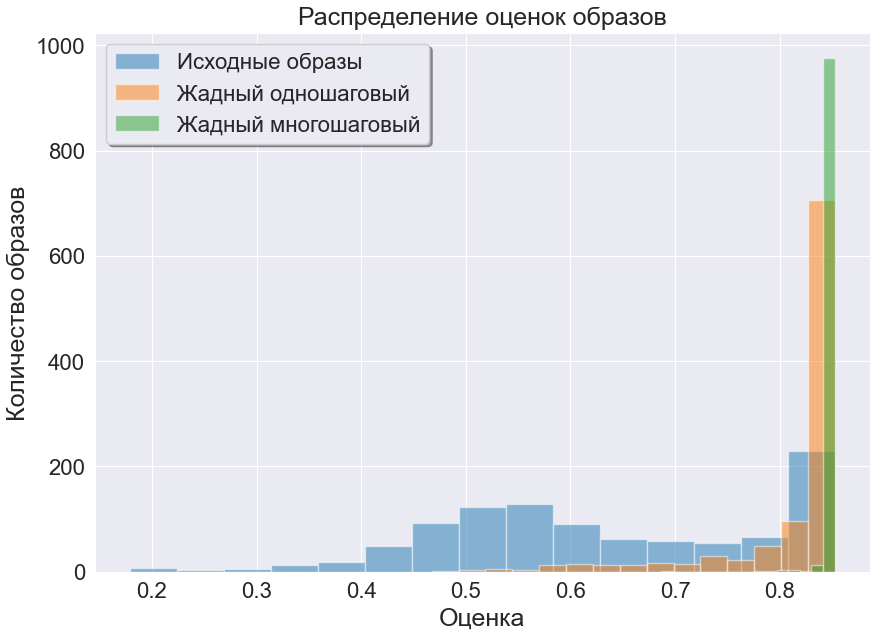
\includegraphics[scale = 0.47]{../figures/greedy_at_least_5_subset1000.png}
		\end{center}
		
		Показывают хороший результат, но требуют слишком много времени
	\end{block}
\end{frame}

\begin{frame}
	\frametitle{Вычислительный эксперимент}
	\begin{block}{Непрерывный подход (градиентный спуск)}
		\vspace{-0.3cm}
		\begin{center}
			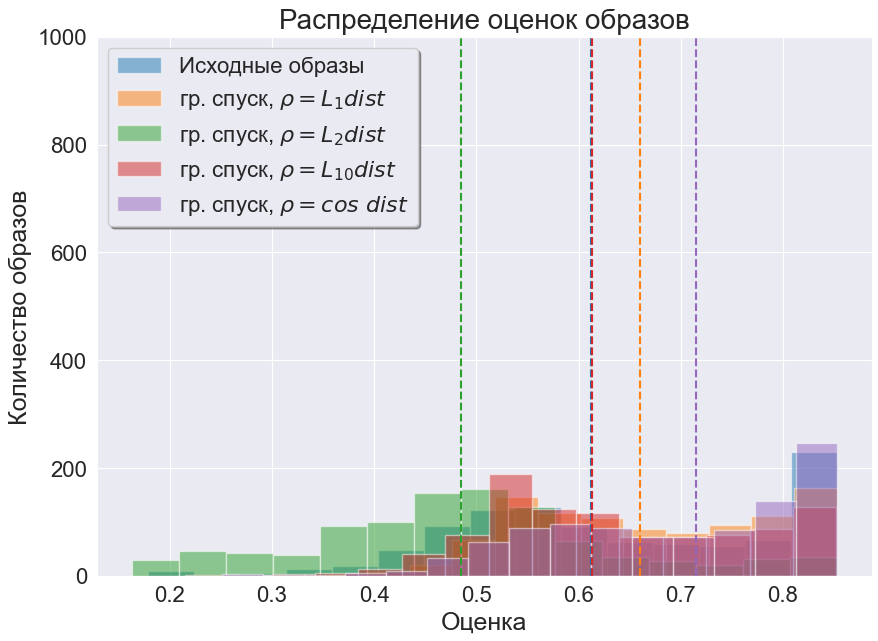
\includegraphics[scale = 0.47]{../figures/backprop_at_least_5_subset1000.png}
		\end{center}
	\end{block}
Результат заметно хуже чем для жадных алгоритмов, а время вычислений еще медленнее, чем ожидалось
\end{frame}

\begin{frame}
	\frametitle{Вычислительный эксперимент}
	\begin{block}{Непрерывный подход (генераций представлений)}
		\vspace{-0.3cm}
		\begin{center}
			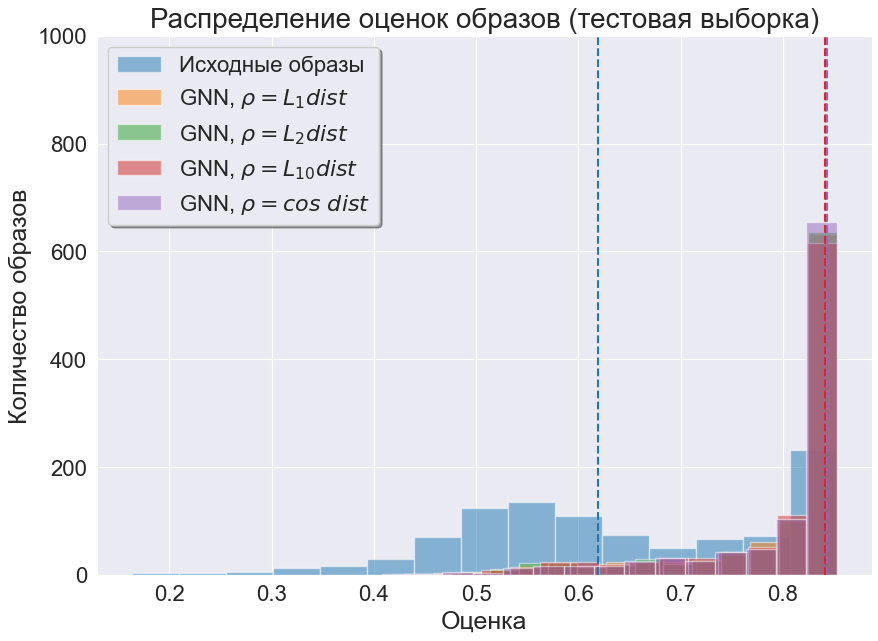
\includegraphics[scale = 0.47]{../figures/GNN_at_least_5_subset1000_test.png}
		\end{center}
	\end{block}
	Качество гораздо выше градиентного спуска, достижимое за десятки миллисекунд. Интересно, что разницы между различными $\rho$ почти нет.
\end{frame}

\begin{frame}
%	\frametitle{Вычислительный эксперимент}
	\begin{block}{Сравнение рассмотренных методов}
%		\vspace{cm}
		\begin{center}
			\begin{tabular}{|c|cccc|}
				\hline
				\multirow{2}{*}{$\rho$} & \multicolumn{4}{c|}{Выборочная медиана оценок образов}                                                                       \\ \cline{2-5} 
				& \multicolumn{1}{c|}{ж. однош.}            & \multicolumn{1}{c|}{ж. многош.}           & \multicolumn{1}{c|}{гр. спуск} & GNN \\ \hline
				$L_1$                   & \multicolumn{1}{c|}{\multirow{4}{*}{0.8511}} & \multicolumn{1}{c|}{\multirow{4}{*}{0.8467}} & \multicolumn{1}{c|}{0.6602}         & 0.8417    \\ \cline{1-1} \cline{4-5} 
				$L_2$                   & \multicolumn{1}{c|}{}                     & \multicolumn{1}{c|}{}                     & \multicolumn{1}{c|}{0.4850}         & 0.8417  \\ \cline{1-1} \cline{4-5} 
				$L_{10}$                & \multicolumn{1}{c|}{}                     & \multicolumn{1}{c|}{}                     & \multicolumn{1}{c|}{0.6132}         &  0.8415  \\ \cline{1-1} \cline{4-5} 
				$cos~dist$              & \multicolumn{1}{c|}{}                     & \multicolumn{1}{c|}{}                     & \multicolumn{1}{c|}{0.7142}         &  0.8428  \\ \hline
				Задержка, с             & \multicolumn{1}{c|}{$\sim$4}                     & \multicolumn{1}{c|}{$\sim$8}                     & \multicolumn{1}{c|}{$\sim$5}          &   $\sim$0.03  \\ \hline
			\end{tabular}
		\end{center}
	
	\end{block}
	\begin{block}{Выводы}
		\begin{enumerate}
		\item Жадные алгоритмы показывают хороший результат, но не применимы на практике. 
		\item Подход с решением релаксированной задачи себя не оправдал --- для данных не выполнено <<условие плотности>>.\\
		\item Генерация представлений существенно быстрее и почти не уступает в качестве.
		\end{enumerate}
	\end{block}
\end{frame}



\begin{frame}
	\frametitle{Выносится на защиту}
		\begin{enumerate}
			\item Предложен и обоснован эффективный алгоритм дополнения образа произвольным числом взаимосвязанных элементов
			\item Предложен способ пополнения обучающих данных для модели в условиях недостатка образов с высокой оценкой
			\item Реализован программный код для вычислительного эксперимента и проведена оценка предложенных подходов				
		\end{enumerate}
\end{frame}




\end{document}
